% Template for IWAENC 2026 paper; to be used with:
%          spconf.sty  - ICASSP/ICIP LaTeX style file, and
%          IEEEbib.bst - IEEE bibliography style file.
% --------------------------------------------------------------------------
\documentclass{article}
\usepackage{spconfa4,amsmath,graphicx,hyperref}

% Title.
% ------
\title{Redes Neuronales en Grafos para Visión por Computadora}
%
% Single address.
% ---------------
\name{Graciana Castro, Julian O'Flaherty}
\address{Aprendizaje Automático para Datos en Grafos, Facultad de Ingeniería, UDELAR}
%

\begin{document}
%\ninept
%
\maketitle
\pagestyle{plain}
\setcounter{page}{1}
%
\begin{abstract}
    % #TODO: completar.

\end{abstract}
%
\begin{keywords}
    Visión por computadora, clasificación de imágenes, redes neuronales en grafos, superpíxeles, conectividad dinámica.
\end{keywords}
%
\section{Introducción}
\label{sec:intro}

Los grafos constituyen una de las herramientas más generales para modelar sistemas complejos, ya que permiten representar entidades y relaciones de manera explícita mediante nodos y aristas. Desde redes sociales y sistemas de transporte hasta interacciones biológicas y estructuras de conocimiento, una gran variedad de fenómenos del mundo real puede formularse naturalmente como un grafo.

La visión por computadora constituye uno de los campos más activos en inteligencia artificial, impulsado por la necesidad de resolver problemas fundamentales como clasificación de imágenes, la segmentación semántica y la detección y seguimiento de objetos \cite{graphs2022}. Estos problemas encuentran aplicaciones en áreas muy diversas como conducción autónoma, diagnóstico médico y robots autónomos. Los desafíos computacionales involucrados como son capturar información visual importante o manejar variabilidad de las imágenes, han impulsado el desarrollo de arquitecturas cada vez más sofisticadas.

En este contexto, los grafos presentan una alternativa a la representación tradicional de las imágenes como grillas: en lugar de tratar la imagen solo como una matriz de píxeles, puede representarse como una estructura relacional donde regiones se conectan según criterios espaciales o de similitud. En este contexto, este informe se centra en la aplicación de redes neuronales sobre grafos (GNNs) a tareas de clasificación de imágenes. En particular, se estudian dos estrategias de modelado: una basada en superpíxeles y otra basada en \textit{patches} con conectividad dinámica.

El primer enfoque \cite{avelar2020superpixel} plantea transformar cada imagen en un \textit{Region Adjacency Graph} (RAG), donde cada nodo representa un superpíxel y las aristas unen regiones vecinas en el plano de la imagen. De esta forma, el grafo preserva relaciones espaciales locales entre regiones semánticamente más homogéneas que los píxeles individuales. Sobre este grafo se entrena un modelo de \textit{Graph Attention Network} (GAT), que actualiza las representaciones de los nodos mediante mecanismos de atención sobre sus vecinos para luego obtener una representación vectorial de toda la imagen. Finalmente, esa representación de grafo se utiliza para predecir la clase presente en la imagen mediante una capa de salida diseñada para clasificación.

En el segundo enfoque \cite{han2022vision} la imagen se divide en \textit{patches} y cada uno se interpreta como un nodo del grafo. La conectividad se define con un criterio de vecinos más cercanos (\textit{k}-NN) en el espacio de características, lo que produce un grafo que puede variar entre capas y adaptarse dinámicamente al contenido visual. La clasificación se realiza a través de bloques que alternan agregación en el grafo y transformación de características, permitiendo combinar información local y global.

La comparación de ambos trabajos resulta interesante porque muestran dos maneras distintas de construir el grafo de entrada: una basada en segmentación espacial explícita (superpíxeles) y otra basada en relaciones de similitud entre \textit{patches}. A lo largo del informe se detallan los modelos, los criterios de construcción de grafos, la configuración experimental empleada y el análisis de resultados en tareas de clasificación de imágenes.

El resto del informe se organiza de la siguiente manera: en la sección \ref{sec:metodologia} se describen las bases de datos utilizadas y los modelos implementados; en la sección \ref{sec:experimentos} se detallan los experimentos realizados; en la sección \ref{sec:resultados} se presentan los resultados obtenidos; finalmente, en la sección \ref{sec:conclusiones} se discuten las conclusiones y posibles líneas futuras de trabajo.

\section{Metodología}
\label{sec:metodologia}
En esta sección se describen las bases de datos utilizadas para evaluar los modelos implementados, así como los detalles de cada modelo, incluyendo la construcción del grafo de entrada y la arquitectura de la red neuronal utilizada para la clasificación.

\subsection{Bases de datos}
\label{subsec:datasets}
Se eligieron cuatro conjuntos de datos clásicos en el trabajo con imágenes que presentan diferentes características y niveles de dificultad y permiten analizar el desempeño de los modelos en distintos escenarios.

\subsubsection{MNIST}
La base de datos MNIST \cite{deng2012mnist} es un conjunto de imágenes de dígitos manuscritos, con 60,000 imágenes de entrenamiento y 10,000 imágenes de prueba. Cada imagen es de tamaño 28x28 píxeles en escala de grises, y el objetivo es clasificar cada imagen en una de las 10 clases correspondientes a los dígitos del cero al nueve. MNIST es un conjunto de datos ampliamente utilizado como punto de partida para evaluar modelos de clasificación de imágenes, debido a su simplicidad y a la gran cantidad de trabajos que lo han utilizado como referencia. En la Figura \ref{fig:mnist_examples} se muestran ejemplos representativos de las imágenes que se pueden encontrar.

\begin{figure}[htb]
    \centering
    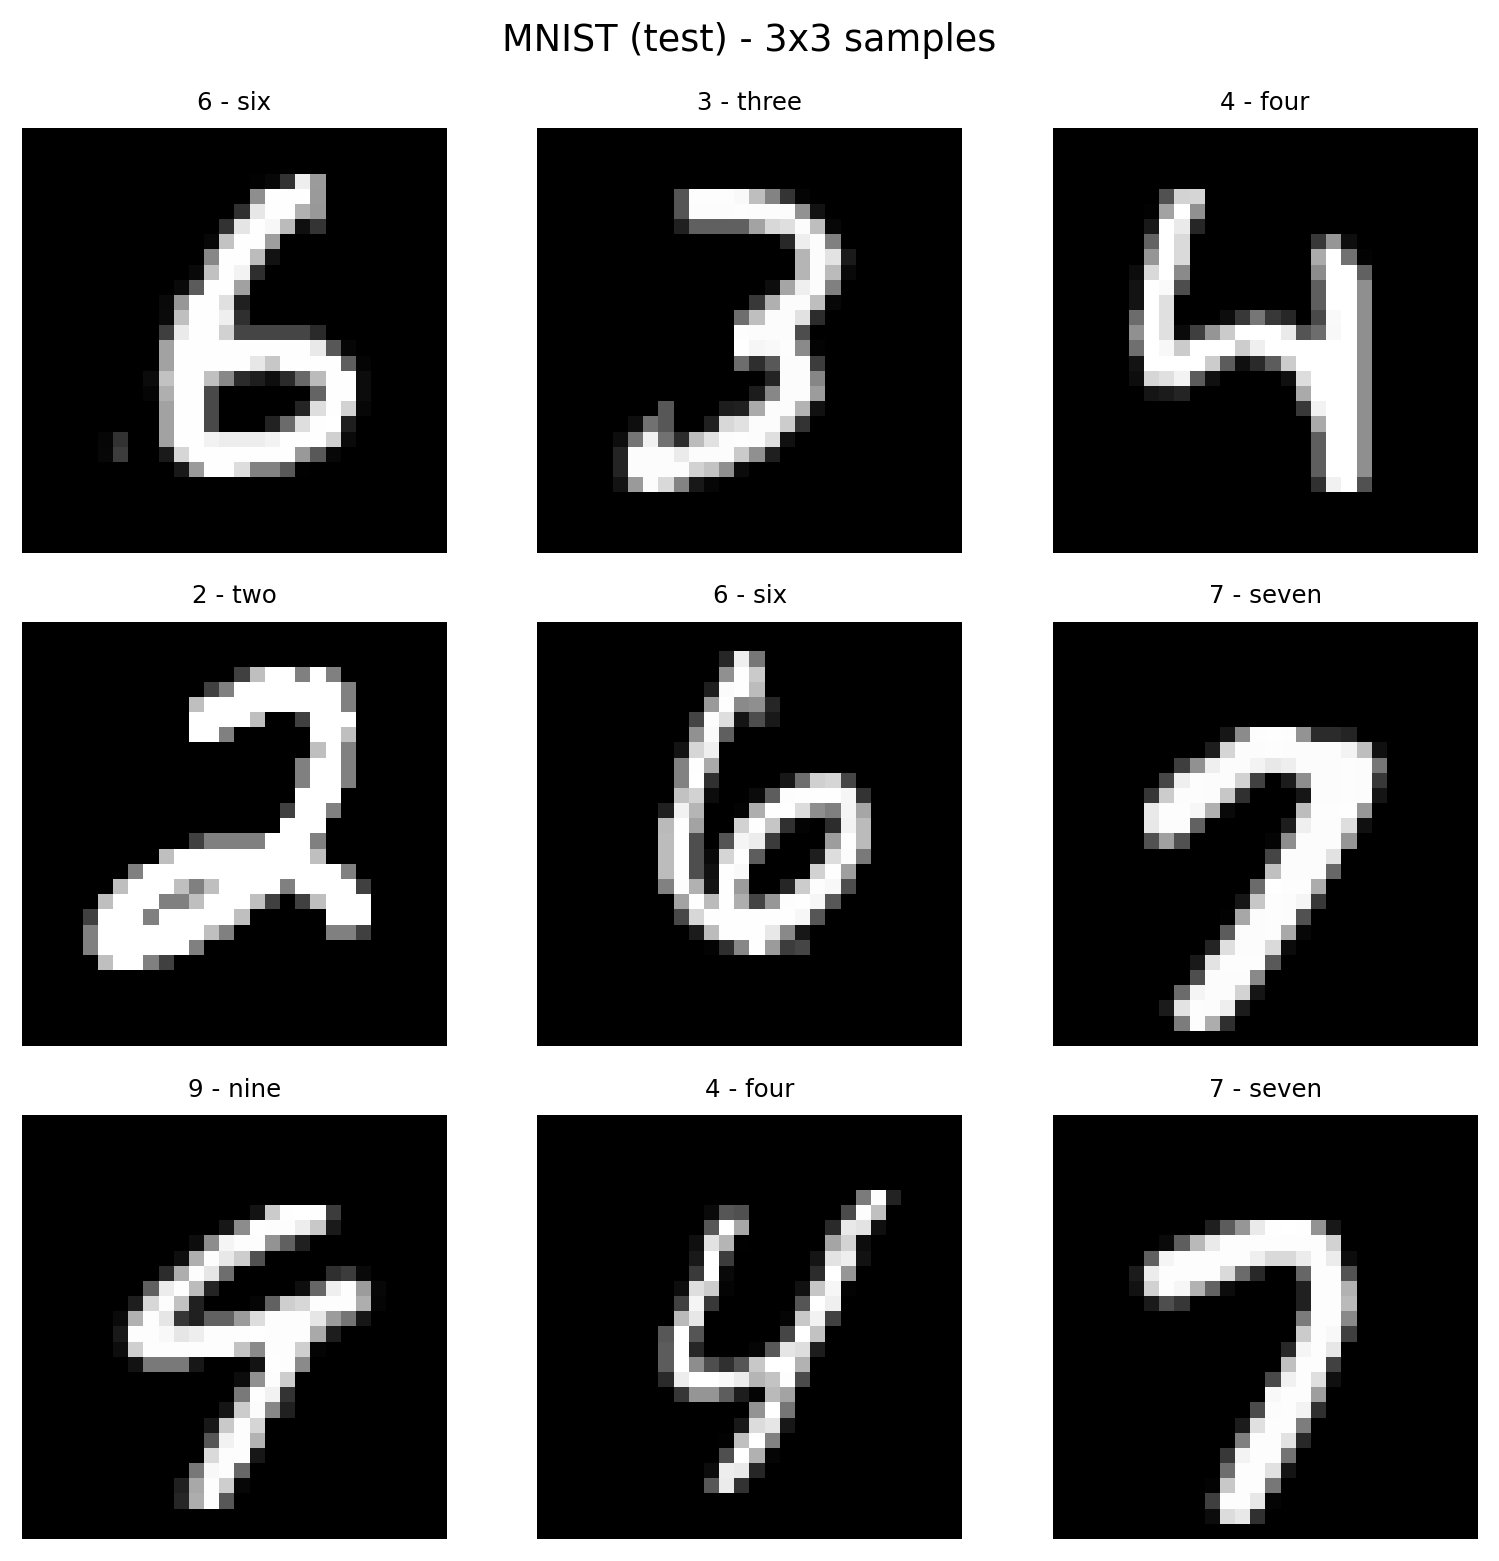
\includegraphics[width=0.85\linewidth]{images/mnist_grid_3x3.png}
    \caption{Ejemplos del conjunto de datos MNIST utilizados en el trabajo.}
    \label{fig:mnist_examples}
\end{figure}

\subsubsection{STL10}
La base de datos STL10 \cite{pmlr-v15-coates11a} contiene un conjunto de imágenes a color (tres canales RGB) de 96x96 píxeles que muestra diez clases de objetos, con 5,000 imágenes de entrenamiento y 8,000 imágenes de prueba. Las clases incluyen aviones, automóviles, pájaros, gatos, ciervos, perros, ranas, caballos, barcos y camiones. STL10 es un conjunto de datos más desafiante que MNIST debido a la mayor complejidad visual y a la presencia de ruido en las imágenes. La Figura \ref{fig:stl10_examples} presenta una muestra ilustrativa de este conjunto.

\begin{figure}[htb]
    \centering
    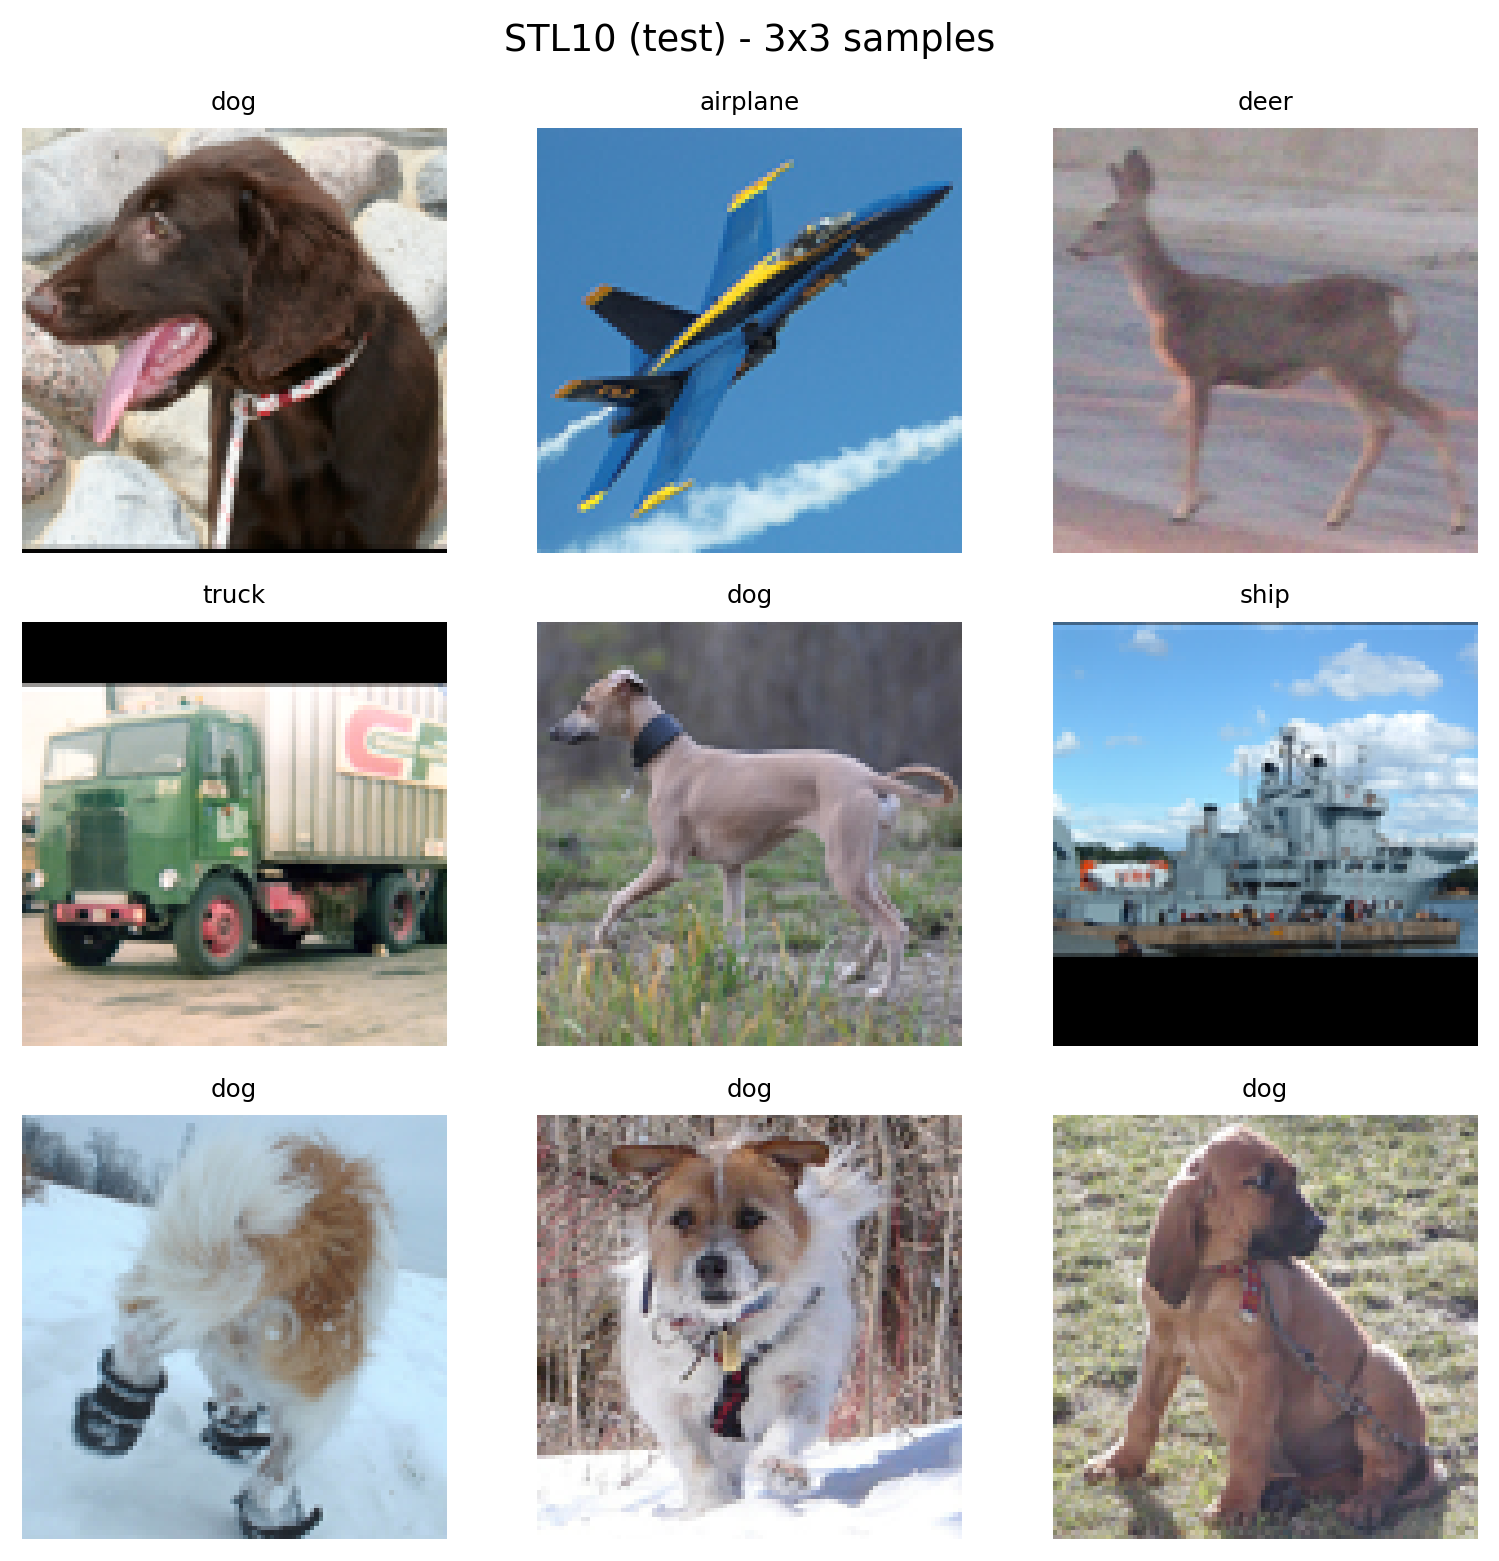
\includegraphics[width=0.85\linewidth]{images/stl10_grid_3x3.png}
    \caption{Ejemplos del conjunto de datos STL10 utilizados en el trabajo.}
    \label{fig:stl10_examples}
\end{figure}

\subsubsection{Imagenet 100 RECORDAR SACAR ESTO SI LA BASE DE DATOS NO SE USAAAAAAAAAA!!!}
La base de datos Imagenet 100 \cite{ILSVRC15} es una versión reducida del conjunto de datos Imagenet, que contiene 100 clases de objetos con un total de 130,000 imágenes. Cada imagen es de alta resolución y a color, y el objetivo es clasificar cada imagen en una de las 100 clases correspondientes. Imagenet 100 es un conjunto de datos muy desafiante debido a la gran variedad de objetos y a la complejidad visual presente en las imágenes.
% #TODO: agregar grilla de imágenes de referencia.

\subsubsection{Pascal VOC0712}
La base de datos Pascal VOC0712 \cite{everingham2010pascal} es un conjunto de datos utilizado principalmente para tareas de segmentación semántica y detección de objetos, pero también se puede adaptar para clasificación. Contiene imágenes a color con una resolución variable, que muestran 20 clases de objetos comunes en escenas cotidianas, como personas, animales, vehículos y muebles. El conjunto de datos se divide en dos partes: VOC2007 con 9963 imágenes y VOC2012 con 11540 imágenes.
% #TODO: agregar grilla de imágenes de referencia.

\subsection{Superpixel GAT}
Se define un superpixel como un grupo de píxeles contiguos que comparten características visuales similares (como color, textura o intensidad). La segmentación en superpíxeles permite reducir la dimensión de la imagen al agrupar píxeles en regiones coherentes, lo que facilita el análisis y la clasificación. Particularmente, se utiliza el método SLIC (Simple Linear Iterative Clustering) \cite{6205760} para segmentar la imagen en superpíxeles. Este método agrupa píxeles en regiones de tamaño similar basándose en la similitud de color y proximidad espacial. El número de superpíxeles se puede ajustar según el nivel de detalle deseado, y cada superpixel se representa mediante un vector de características que puede incluir información como el color promedio, la textura o la forma.

Una vez segmentada la imagen en superpíxeles, se construye un grafo de adyacencia de regiones (RAG) donde cada nodo representa un superpixel y las aristas conectan nodos que corresponden a superpíxeles adyacentes en la imagen. Este grafo captura las relaciones espaciales entre las regiones segmentadas, lo que permite al modelo aprender patrones de interacción entre diferentes partes de la imagen. Las Figuras \ref{fig:mnist_superpixel_rag_examples} y \ref{fig:stl10_superpixel_rag_examples} muestran ejemplos de grafos RAG generados sobre imágenes de MNIST y STL10 usando SLIC.

\begin{figure}[htb]
    \centering
    \small
    \fbox{\parbox[c][0.9cm][c]{1.6cm}{\centering Imagen}}
    $\rightarrow$
    \fbox{\parbox[c][0.9cm][c]{1.9cm}{\centering SLIC}}
    $\rightarrow$
    \fbox{\parbox[c][0.9cm][c]{2.0cm}{\centering Grafo RAG}}
    $\rightarrow$
    \fbox{\parbox[c][0.9cm][c]{2.2cm}{\centering Capas GAT}}
    $\rightarrow$
    \fbox{\parbox[c][0.9cm][c]{2.3cm}{\centering Agregación global}}
    $\rightarrow$
    \fbox{\parbox[c][0.9cm][c]{1.5cm}{\centering MLP + softmax}}
    \caption{Esquema del pipeline de clasificación del enfoque Superpixel-GAT.}
    \label{fig:superpixel_gat_pipeline}
\end{figure}

El flujo general del modelo utilizado para clasificación se resume en la Figura \ref{fig:superpixel_gat_pipeline}.

\begin{figure}[htb]
    \centering
    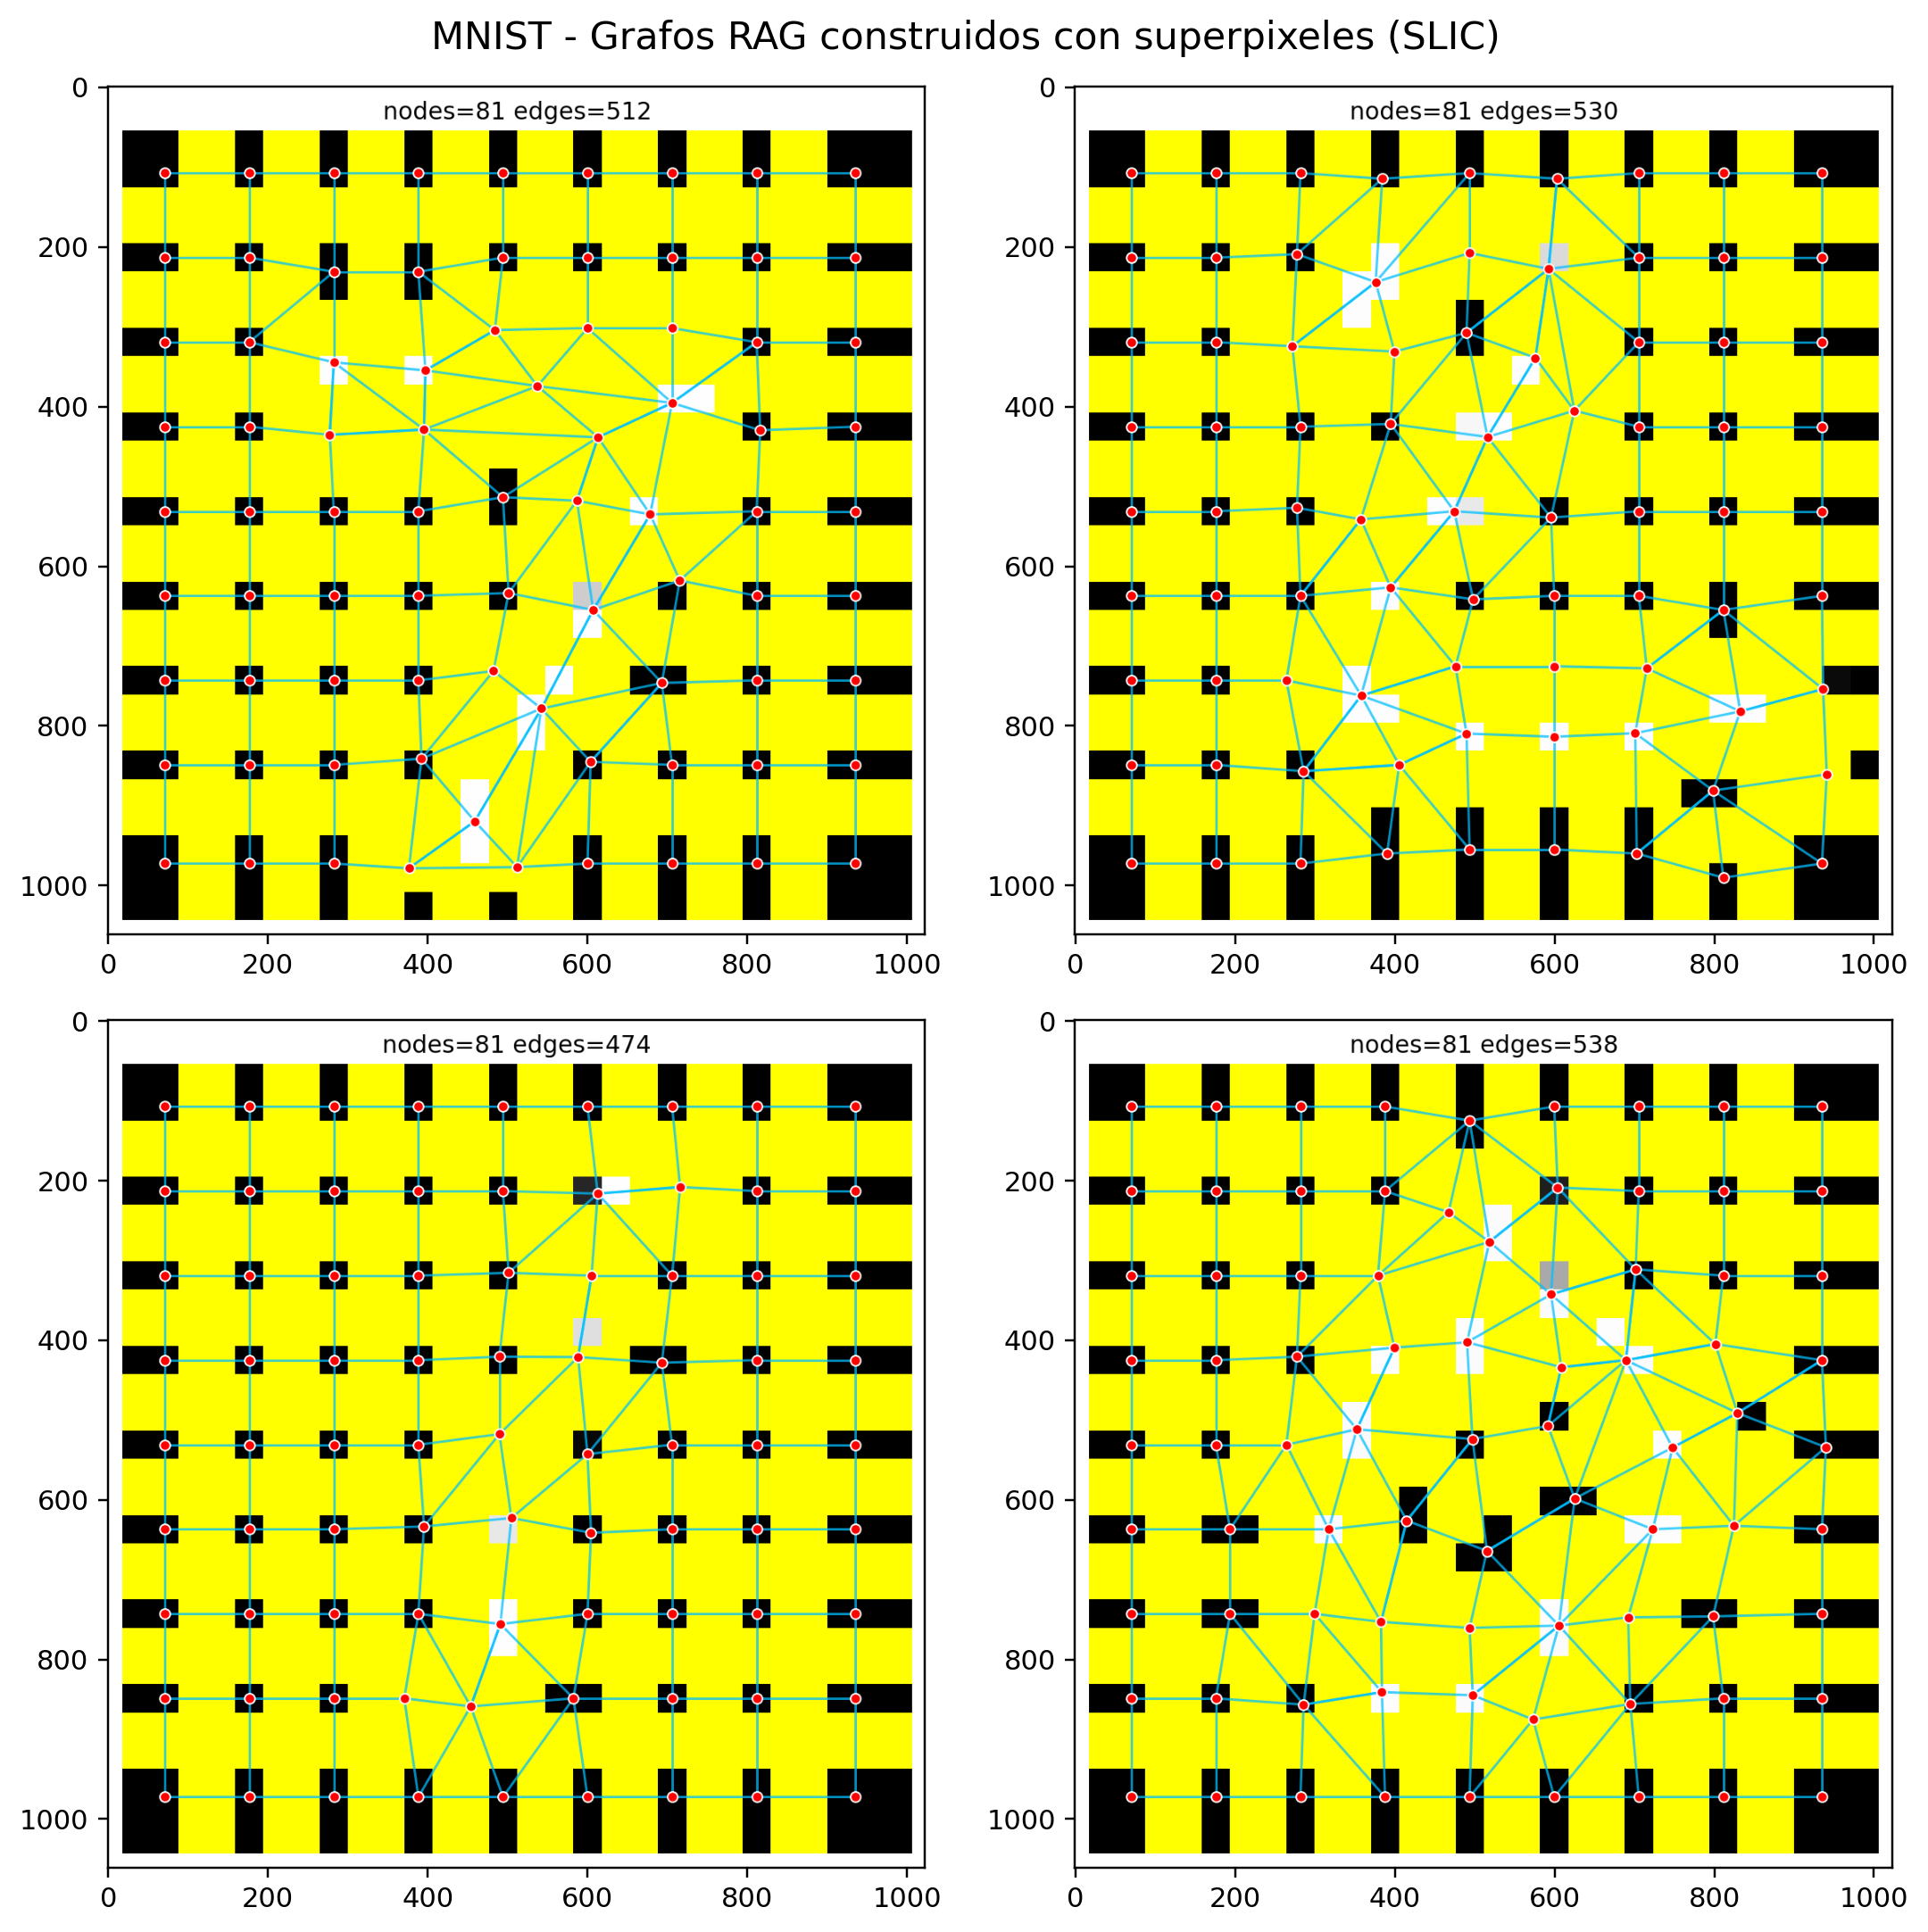
\includegraphics[width=0.98\linewidth]{images/mnist_superpixel_rag_grid_2x2.png}
    \caption{Ejemplos de grafos RAG construidos a partir de superpíxeles en MNIST mediante SLIC.}
    \label{fig:mnist_superpixel_rag_examples}
\end{figure}

\begin{figure}[htb]
    \centering
    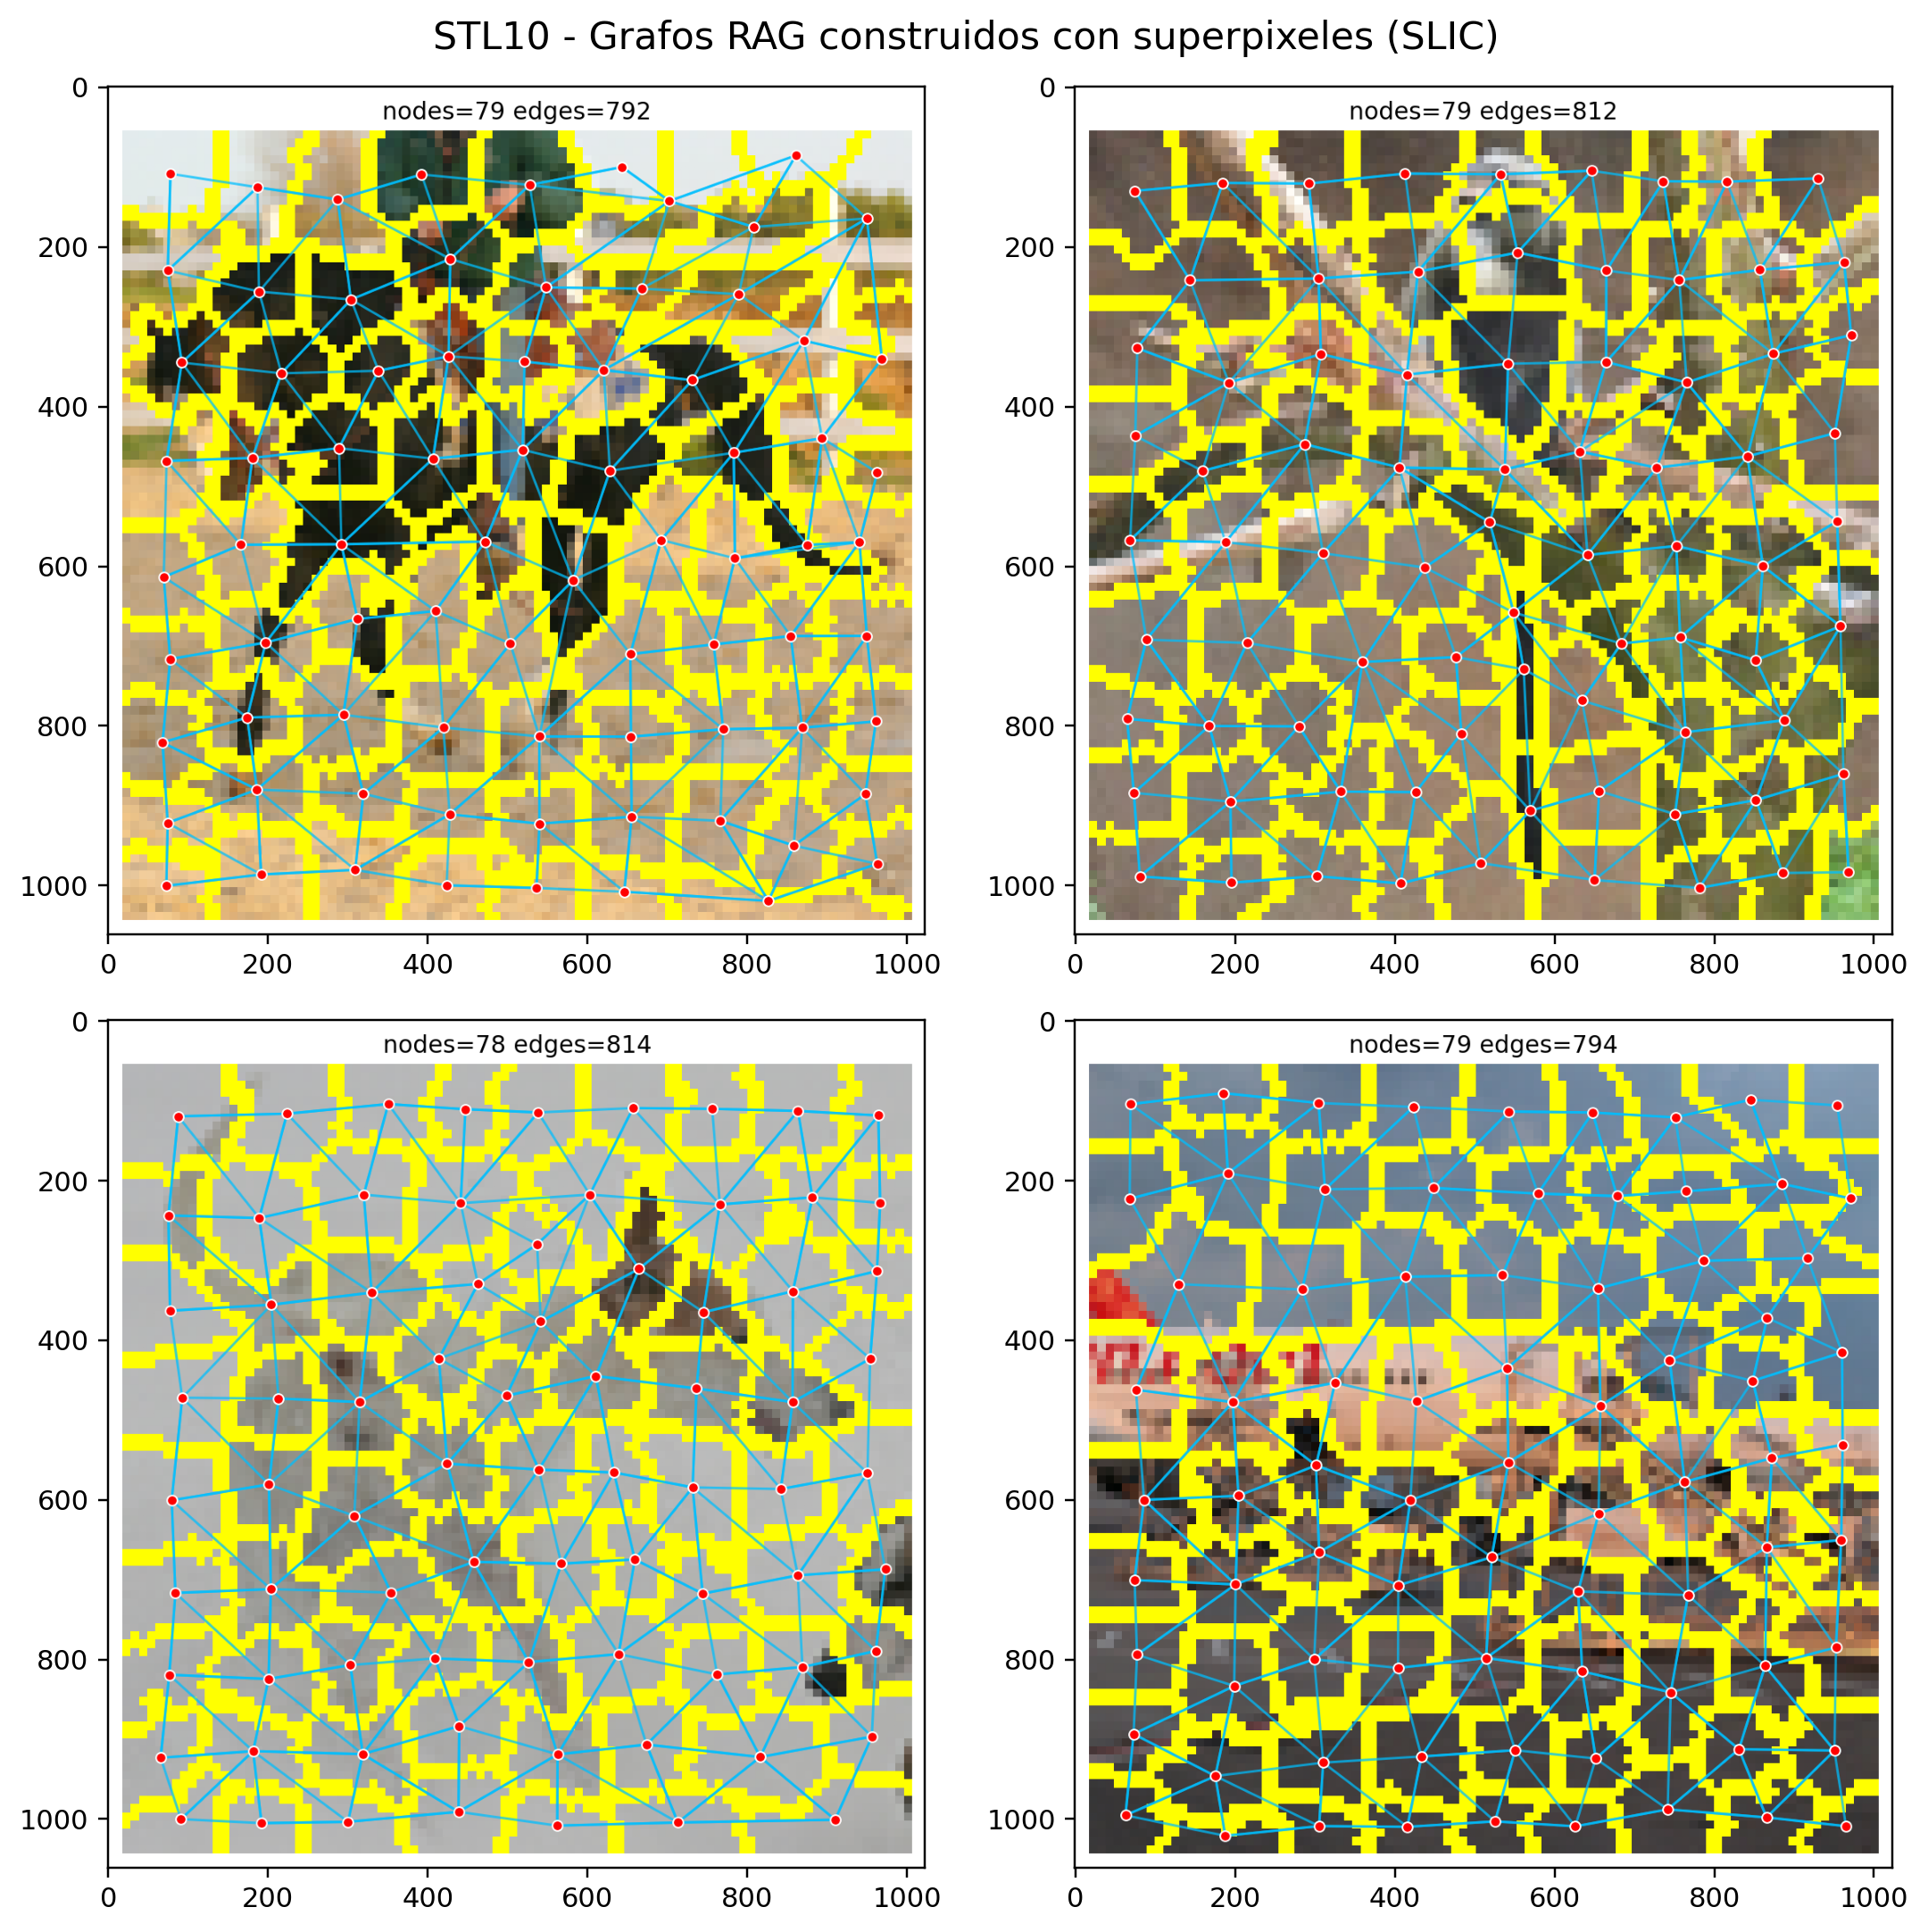
\includegraphics[width=0.98\linewidth]{images/stl10_superpixel_rag_grid_2x2.png}
    \caption{Ejemplos de grafos RAG construidos a partir de superpíxeles en STL10 mediante SLIC.}
    \label{fig:stl10_superpixel_rag_examples}
\end{figure}

Para la clasificación, se utiliza una GAT \cite{velickovic2018graph}, que actualiza las representaciones de los nodos mediante mecanismos de atención sobre sus vecinos. En cada capa, primero se aplica una transformación lineal a las características de los nodos y luego se calcula, para cada arista $(i,j)$, un coeficiente de atención no normalizado:
\begin{equation}
    e_{ij} = \text{LeakyReLU}\left(\mathbf{a}^{\top}[\mathbf{W}\mathbf{h}_i\,\|\,\mathbf{W}\mathbf{h}_j]\right)
\end{equation}
donde $\mathbf{h}_i$ es la representación del nodo $i$, $\mathbf{W}$ son parámetros entrenables y $\mathbf{a}$ es el vector de atención.

Luego, estos coeficientes se normalizan con \textit{softmax} sobre el vecindario de cada nodo:
\begin{equation}
    \alpha_{ij} = \frac{\exp(e_{ij})}{\sum_{k \in \mathcal{N}(i)} \exp(e_{ik})}
\end{equation}
y la nueva representación del nodo se obtiene como una suma ponderada de vecinos:
\begin{equation}
    \mathbf{h}'_i = \sigma\left(\sum_{j \in \mathcal{N}(i)} \alpha_{ij}\,\mathbf{W}\mathbf{h}_j\right)
\end{equation}

En el caso particular de superpíxeles, estos pesos de atención permiten que el modelo priorice regiones vecinas más informativas para la clasificación de la imagen completa. Finalmente, a partir de las representaciones de cada superpixel se obtiene una representación vectorial global que se utiliza en una capa lineal con \textit{softmax} para predecir la clase.

\subsection{VisionGNN}

\subsubsection{Red isotrópica}

\subsubsection{Red piramidal}

\section{Experimentos}
\label{sec:experimentos}
Para evaluar el desempeño de los modelos presentados, se realizaron entrenamientos y pruebas utilizando las bases de datos descritas en la sección \ref{subsec:datasets}. Las pruebas se llevaron a cabo basadas en el código de github de cada trabajo \footnote{\href{https://github.com/jichengyuan/Vision_GNN}{https://github.com/jichengyuan/Vision\_GNN}} \footnote{\href{https://github.com/machine-reasoning-ufrgs/spixel-gat}{https://github.com/machine-reasoning-ufrgs/spixel-gat}}. Además, se entrenó una Resnet-18 \cite{resnet} como baseline para comparar el desempeño de los modelos basados en grafos con una arquitectura de red neuronal para clasificación de imágenes tradicional.

\section{Resultados}
\label{sec:resultados}

\section{Conclusiones}
\label{sec:conclusiones}

\section{References}
\label{sec:ref}

En esta sección se listan las referencias bibliográficas del trabajo.

% References should be produced using the bibtex program from suitable
% BiBTeX files (here: strings, refs, manuals). The IEEEbib.bst bibliography
% style file from IEEE produces unsorted bibliography list.
% -------------------------------------------------------------------------
\bibliographystyle{IEEEbib}
\bibliography{refs}

\end{document}
